\documentclass[11pt,a4paper,notitlepage]{article}

\usepackage[T1]{fontenc}
\usepackage[utf8]{inputenc}
\usepackage[english]{babel}
\usepackage{fullpage}
\usepackage{amsmath}
\usepackage{amsfonts}
\usepackage{amssymb}
\usepackage{verbatim}
\usepackage{listings}
\usepackage{color}
\usepackage{setspace}
\usepackage{epstopdf}
\usepackage{graphicx}
\usepackage{caption}
\usepackage{subcaption}
\usepackage{float}
\usepackage{epstopdf}
\usepackage{hyperref}
\usepackage{dsfont}
\usepackage{braket}
\pagenumbering{arabic}

\definecolor{codepurple}{rgb}{0.58,0,0.82}
\definecolor{backcolour}{rgb}{0.95,0.95,0.92}
\definecolor{dkgreen}{rgb}{0,0.6,0}
\definecolor{gray}{rgb}{0.5,0.5,0.5}
\definecolor{mauve}{rgb}{0.58,0,0.82}
%\setlength{\parindent}{0pt}

\lstdefinestyle{pystyle}{
  language=Python,
  aboveskip=3mm,
  belowskip=3mm,
  columns=flexible,
  basicstyle={\small\ttfamily},
  backgroundcolor=\color{backcolour},
  commentstyle=\color{dkgreen},
  keywordstyle=\color{magenta},
  numberstyle=\tiny\color{gray},
  stringstyle=\color{codepurple},
  basicstyle=\footnotesize,  
  breakatwhitespace=false
  breaklines=true,
  captionpos=b,
  keepspaces=true,
  numbers=left,
  numbersep=5pt,
  showspaces=false,
  showstringspaces=false,
  showtabs=false,
  tabsize=2
}
\lstdefinestyle{iStyle}{
  language=IDL,
  aboveskip=3mm,
  belowskip=3mm,
  columns=flexible,
  basicstyle={\small\ttfamily},
  backgroundcolor=\color{backcolour},
  commentstyle=\color{dkgreen},
  keywordstyle=\color{magenta},
  numberstyle=\tiny\color{gray},
  stringstyle=\color{codepurple},
  basicstyle=\footnotesize,  
  breakatwhitespace=false
  breaklines=true,
  captionpos=b,
  keepspaces=true,
  numbers=left,
  numbersep=5pt,
  showspaces=false,
  showstringspaces=false,
  showtabs=false,
  tabsize=2
}
\lstdefinestyle{c++style}{
  language=C++,
  keywordstyle=\color{blue}\ttfamily,
  stringstyle=\color{red}\ttfamily,
  commentstyle=\color{green}\ttfamily,
  morecomment=[l][\color{magenta}]{\#}
  aboveskip=3mm,
  belowskip=3mm,
  columns=flexible,
  basicstyle={\small\ttfamily},
  backgroundcolor=\color{backcolour},
  numberstyle=\tiny\color{gray},
  basicstyle=\footnotesize,  
  breakatwhitespace=false
  breaklines=true,
  captionpos=b,
  keepspaces=true,
  numbers=left,
  numbersep=5pt,
  showspaces=false,
  showstringspaces=false,
  showtabs=false,
  tabsize=2
}

\title{\normalsize Ast4310: - Radiative processes in astrophysics \\
\vspace{10mm}
\huge Stellar Spectra B: LTE Line formation\\
\vspace{10mm}
\normalsize Due date {\bf Nov $11^\text{th}$, 2016}}

% Skriv namnet ditt her og fjern kommenteringa
\author{Magnus Christopher Bareid \\ un: magnucb }

\newcommand{\SE}{Schr\"odinger equation}
\newcommand{\laplacian}{\vec{\nabla}^2}
\newcommand{\eye}{\mathds{I}}
\newcommand\pd[2]{\frac{\partial #1}{\partial #2}}
\def\doubleunderline#1{\underline{\underline{#1}}}


\begin{document}
\noindent
\maketitle
\vspace{5mm}

\begin{figure}[H]
	\centering	
	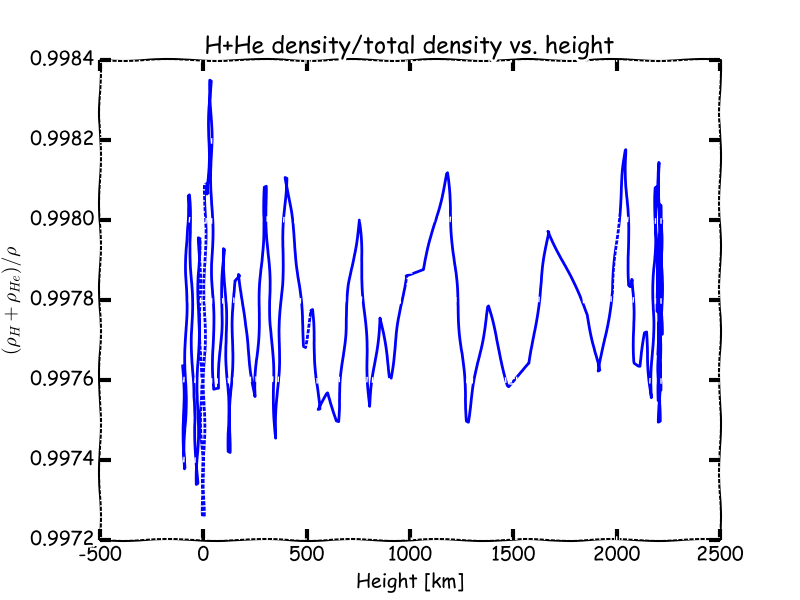
\includegraphics[scale=0.45]{frontpage.png}
\end{figure}
\begin{abstract}
This project specializes the student's knowledge base to include how to treat spectral extinction line formations, by looking at different data pools that are either observed or computed in the distant past and made available for educational purposes.

The assignment then sets out to plot and compare these data, to let the student explain some noteworthy physical phenomena that arise through the data and through numerical models that the student is to implement.
\end{abstract}

%\begin{center}
%\line(1,0){450}
%\end{center}

\newpage
\tableofcontents

\newpage
\section*{Introduction}
First and foremost, we will look at data collected and modeled into the FALC-model and review this data.

After that, this data will be compared to Earth's atmosphere to see how physical phenomena may manifest themselves differently in these two locations.

We will then look at additional data that concerns the Sun's intensities and review this with different models.

Lastly, we will compute an actual physical phenomena, a spectral extinction line from an element that is present in the Sun's atmosphere, and then compare it to actual extinction data.

\section{Stratification of the solar atmosphere} 						%%% section 1

\subsection{FALC temperature stratification}
\begin{figure}[H]
\center
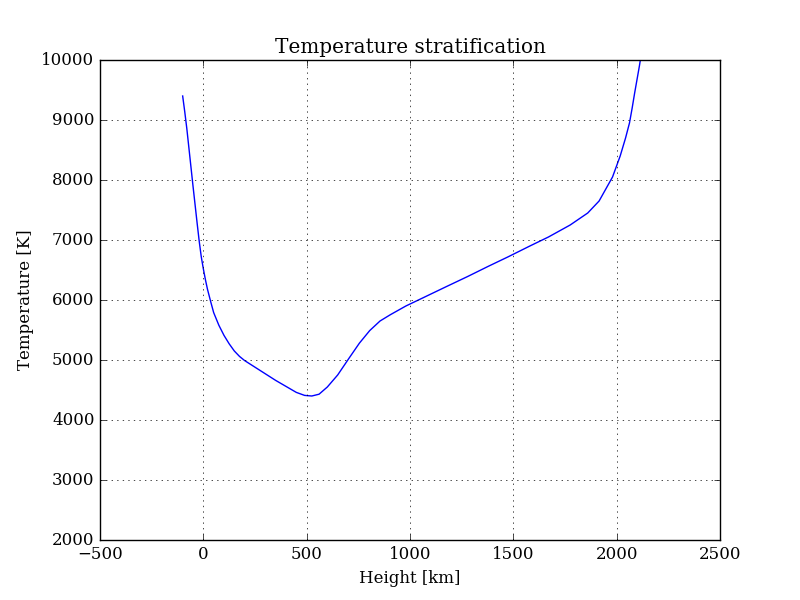
\includegraphics[scale=0.42]{../figs/temp_vs_h.png}
\caption{Plot of temperature stratification.}
\end{figure}


\subsection{FALC density stratification}

\subsubsection{Total pressure against column mass}
\begin{figure}[H]
\center

	\begin{subfigure}{0.49\textwidth}
	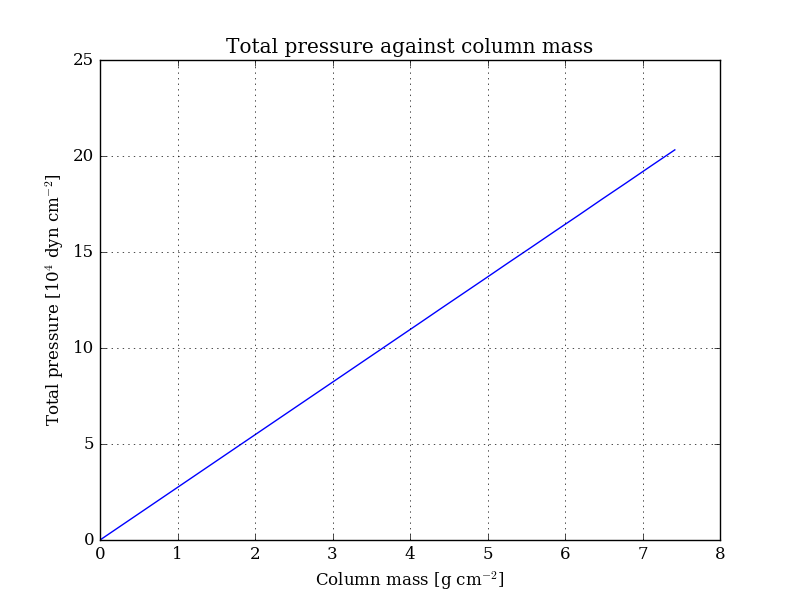
\includegraphics[scale=0.42]{../figs/totpress_vs_m.png}
	\caption{Plot of total pressure against column mass, linearly scaled.}
	\end{subfigure}
	\hfill
	\begin{subfigure}{0.49\textwidth}
	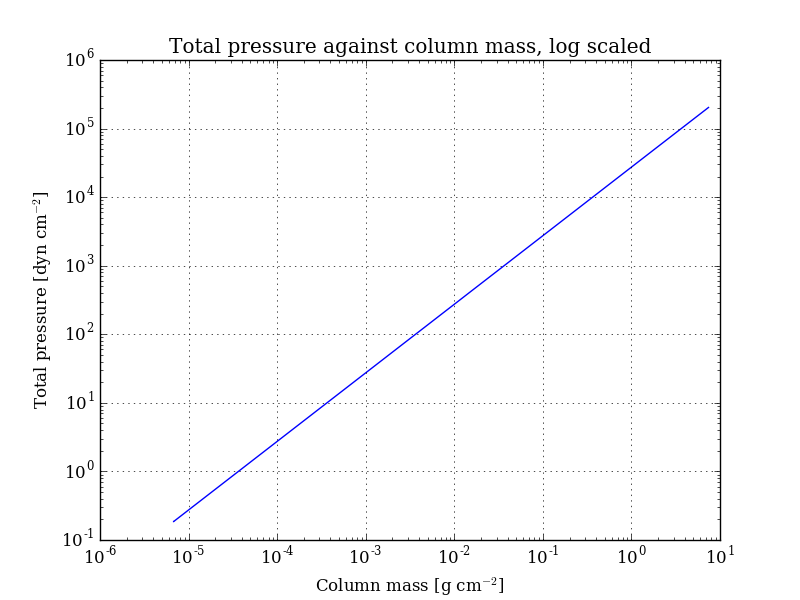
\includegraphics[scale=0.42]{../figs/totpress_vs_m_log.png}
	\caption{Plot of total pressure against column mass, logarithmically scaled.}
	\end{subfigure}

\caption{Pressure plots against column masses with different scalings. What one is able to see here, is that the pressure $p_\text{total}$ scales linearly in such a way that $p_\text{total} = c m_c$, where $c$ is a constant and $m_c$ is column mass. Then, comparing the units of the variables one may derive the relation: $[\frac{p_\text{total}}{m_c}] = [c] = \frac{ \frac{\text{kg m}}{\text{m$^2$s$^2$}} }{\frac{\text{kg}}{\text{m}^2}} = \frac{\text{m}}{\text{ s}^2}$, which are the units of acceleration. If then the scale of the height in which our data is present compared to the Sun's total radius is taken into account (the height we're dealing with is less than half a per cent of the Sun's total radius), one could safely assume that for such a small height differential the gravitational acceleration would remain constant.}
\end{figure}

\subsubsection{Complete mixing at heights}

\begin{figure}[H]
\center

	\begin{subfigure}{0.49\textwidth}
	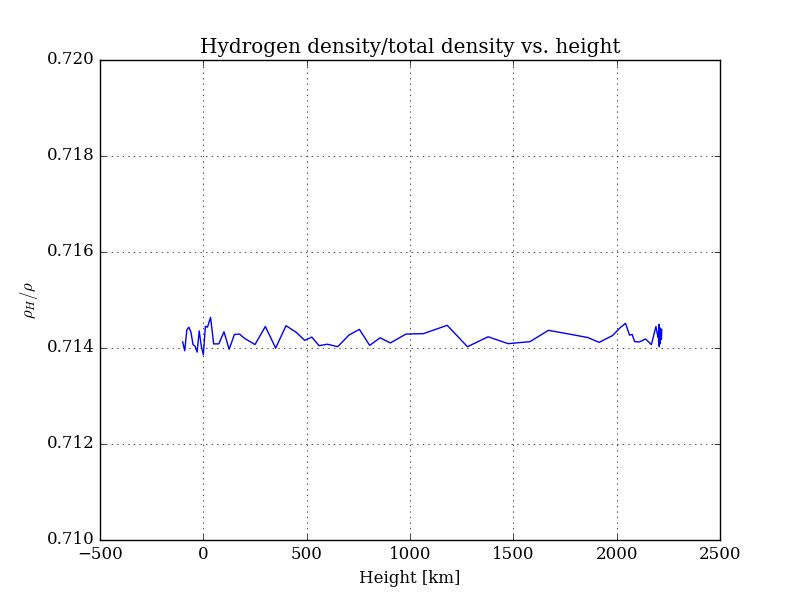
\includegraphics[scale=0.42]{../figs/ratio_Hmassdens_of_dens_vs_h.png}
	\caption{Ratio of hydrogen mass density to total mass density against height.}
	\end{subfigure}
	\hfill
	\begin{subfigure}{0.49\textwidth}
	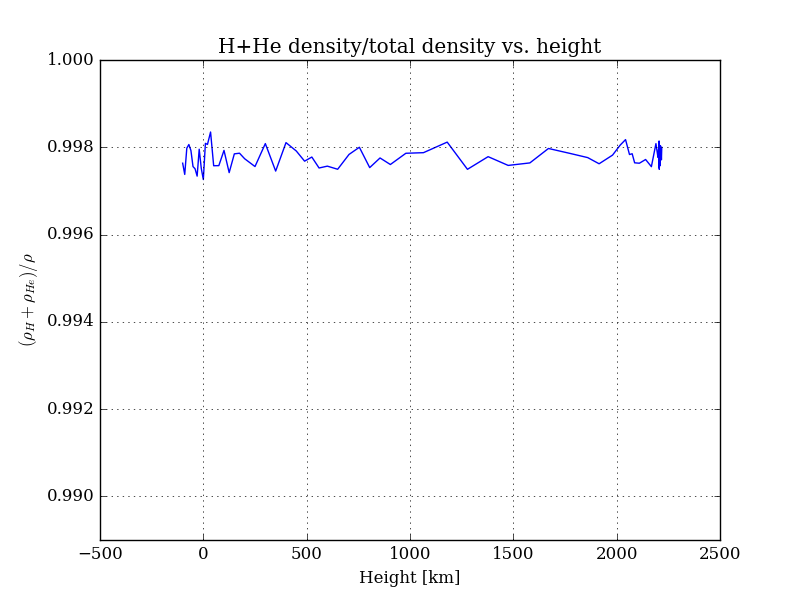
\includegraphics[scale=0.42]{../figs/ratio_HHemassdens_of_dens_vs_h.png}
	\caption{Ratio of hydrogen mass density and helium mass density to total mass density against height.}
	\end{subfigure}

\caption{Ratios of elements' presence over heights. As visible from (b), there is less than 0.2\% of the ratio available for other elements than hydrogen and helium. The ratios seem almost constant, only varying by tiny fraction over the heights which FALC data covers, implying that the elements involved - hydrogen, helium, and metals - are homogeneously mixed through the data's height scale.}
\end{figure}

\subsubsection{Column mass and height}

\begin{figure}[H]
\center

	\begin{subfigure}[t]{0.49\textwidth}
	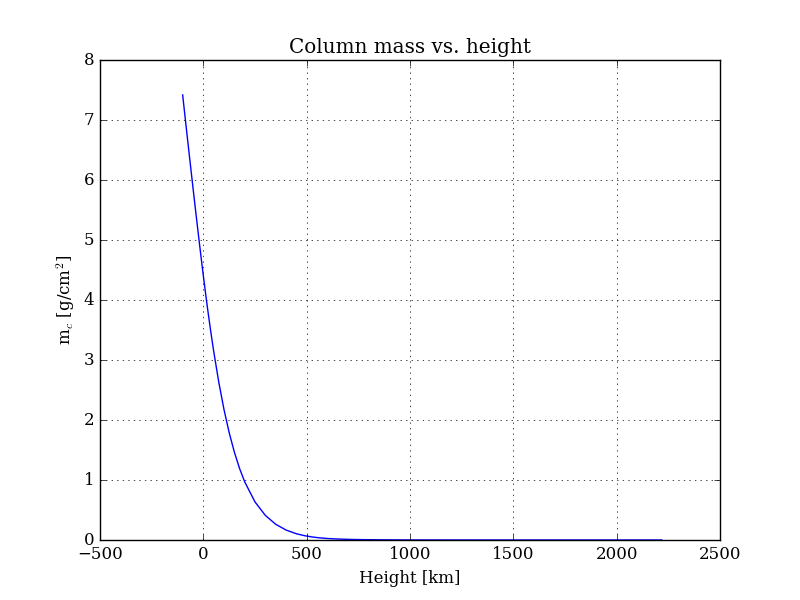
\includegraphics[scale=0.42]{../figs/colm_vs_h.png}
	\caption{Column mass against height, linearly scaled.}
	\end{subfigure}
	\hfill	
	\begin{subfigure}[t]{0.49\textwidth}
	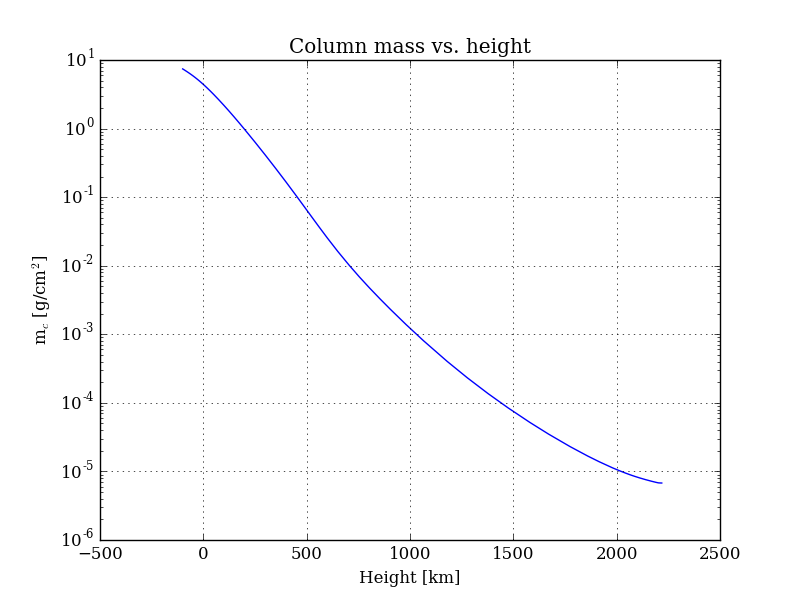
\includegraphics[scale=0.42]{../figs/colm_vs_h_log.png}
	\caption{Column mass against height, logarithmically scaled.}
	\end{subfigure}
	
\caption{Plots of column masses against height with different scalings. If the column mass $m_c$ were logarithmically linear, a mathematical expression to its graph's behaviour would be something along the line of $log(m_c) = a h + b$, where $a, b$ are physical constants and $h$ is height. If one would try to make this approximation for (b)'s line, it seems apparent that it would be a good approximation for an area of the curve at least around $h \in [0, 1500]$ or somewhere around that. The linear approximation seems to break down, given the nature of the curve, outside of these boundaries. It may, however be a part of the final solution to the problem, but on its own the simple logarithmic expression doesn't tell the whole story.}
\end{figure}

\subsubsection{Gas density and height}
\begin{figure}[H]
\center

	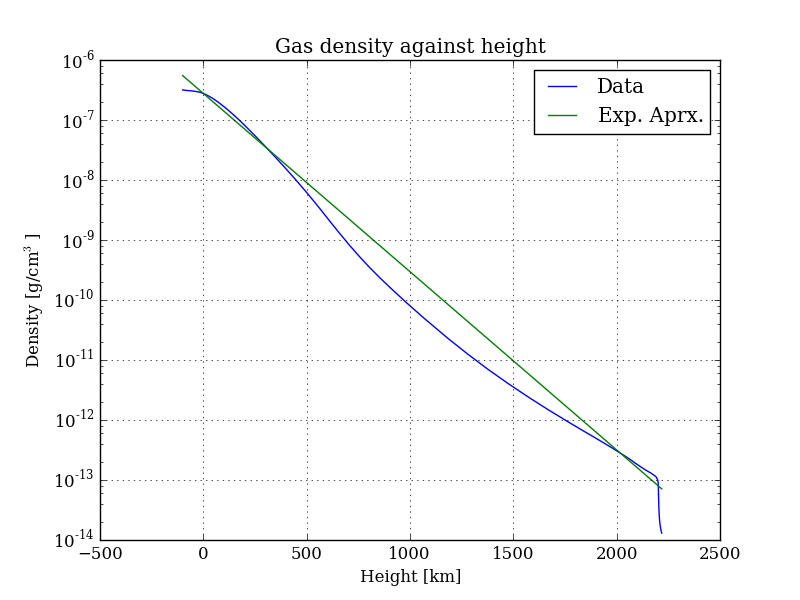
\includegraphics[scale=0.42]{../figs/gasdens_vs_h.png}
	\caption{Gas density and its exponential approximation against height, logarithmically scaled.\\ Density scale height $H_\rho$ may be derived from observing two points of the graph, in whose area the graphs seems to be logarithmically linear, and interconnecting them using an exponential expression.}
\end{figure}
\begin{align}
\rho_{h_1} &= \rho_{h_0} e^{ -\frac{h_1}{H_\rho} } \quad , h_0 = 0 \nonumber \\ 
\frac{\rho_{h_1}}{\rho_{h_0}} &= e^{ -\frac{h_1}{H_\rho} } \nonumber\\ 
- \frac{h_1}{H_\rho} &= ln\left( \frac{\rho_{h_1}}{\rho_{h_0}} \right) \nonumber \\
H_\rho &= \frac{h_1}{ ln\left( \frac{\rho_{h_0}}{\rho_{h_1}} \right) }
\end{align}

\subsubsection{Gas pressure and height}

\begin{figure}[H]
\center

	\begin{subfigure}[t]{0.49\textwidth}
	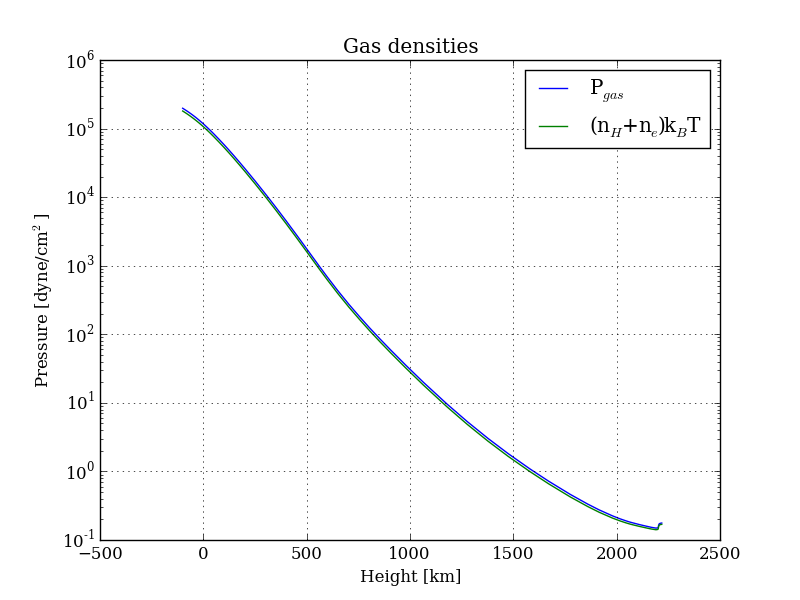
\includegraphics[scale=0.42]{../figs/gasP_vs_h.png}
	\caption{Gas pressure and ideal gas pressure, against height, log scaled.}
	\end{subfigure}
	\hfill	
	\begin{subfigure}[t]{0.49\textwidth}
	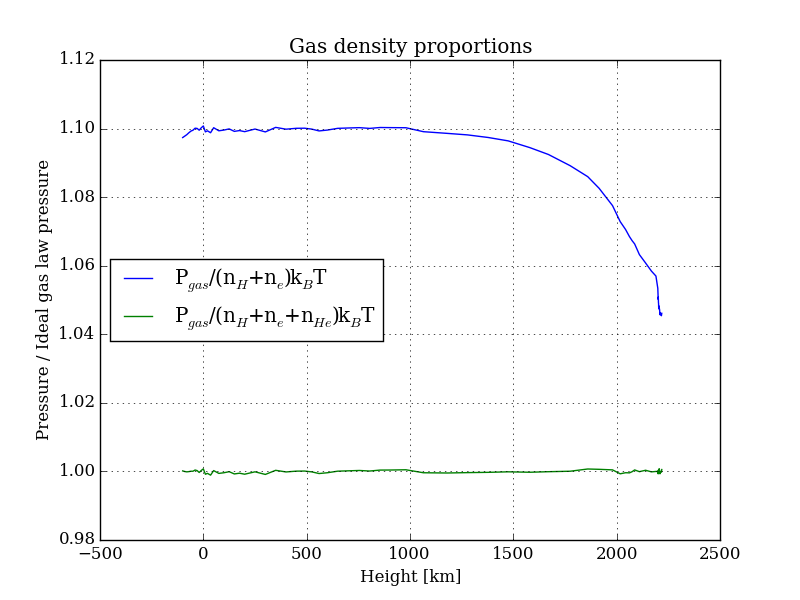
\includegraphics[scale=0.42]{../figs/gasP_vs_h_ideal.png}
	\caption{Ratios of gas pressure over ideal gas pressure, and gas pressure with helium taken into account, against height.}
	\end{subfigure}
	
\caption{Plots of gas density and their ratios, compared with ideal gas laws, against height with different scalings. \\ The differences make total sense. The FALC gas pressure is too great compared with ideal gas law, if the ideal gas does not consider the presence of helium as an element in the mix of gases in the Sun. The green line in (b) then shows how well the ideal gas law approximates FALC data, as long as helium is included in the model.}
\end{figure}

\subsubsection{Density comparisons}

\begin{figure}[H]
\center

	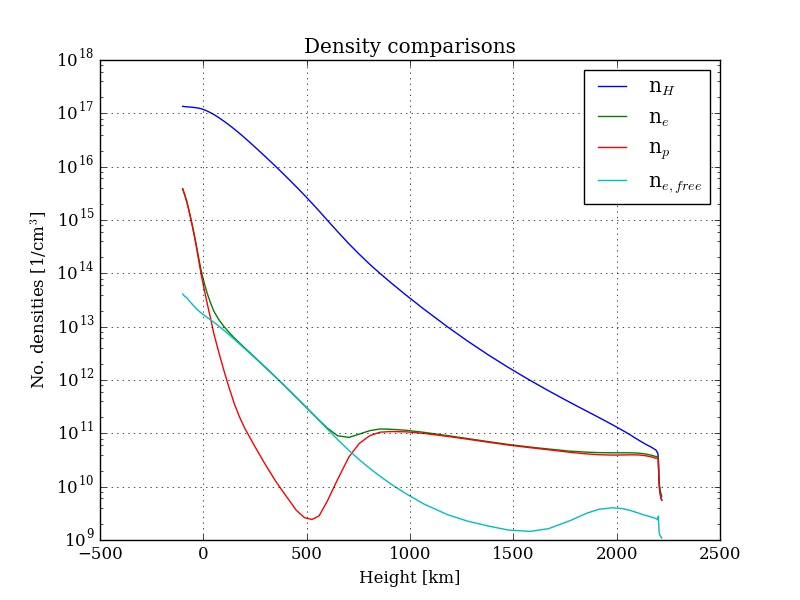
\includegraphics[scale=0.42]{../figs/dens_comp.png}
	\caption{Plot of number densities for basic constituents of the Sun's gas over a height range.\\
	It is somewhat obvious that all densities decrease with increasing height; the atomized hydrogen having the most stable curve to illustrate this. The dip at large height, on the end of all the curves is notable, probably suggesting a surface feature of some kind.\\
	As height increases, the free proton density goes down dramatically, implying that the ratio between hydrogen atoms (protons bound with an electron) and free protons is increasing for a height range, until the free protons' number desnity increases again, suggesting that hydrogen becomes more ionized at this height as the hydrogen density continues to decrease.\\
	In the height range where free protons' density decreases compared to hydrogen density (and for a tiny bit onwards), the free electron density (not from ionized hydrogen) is parallel to the hydrogen density. This implies that the ratio between these free electrons and hydrogen are constant, and decrease with height as a homogeneous mix for the aforementioned height range, in contrast with the other number densities that increase and decrease more varyingly because of underlying physical processes.}
\end{figure}


\subsubsection{Ionization fraction}

\begin{figure}[H]
\center

	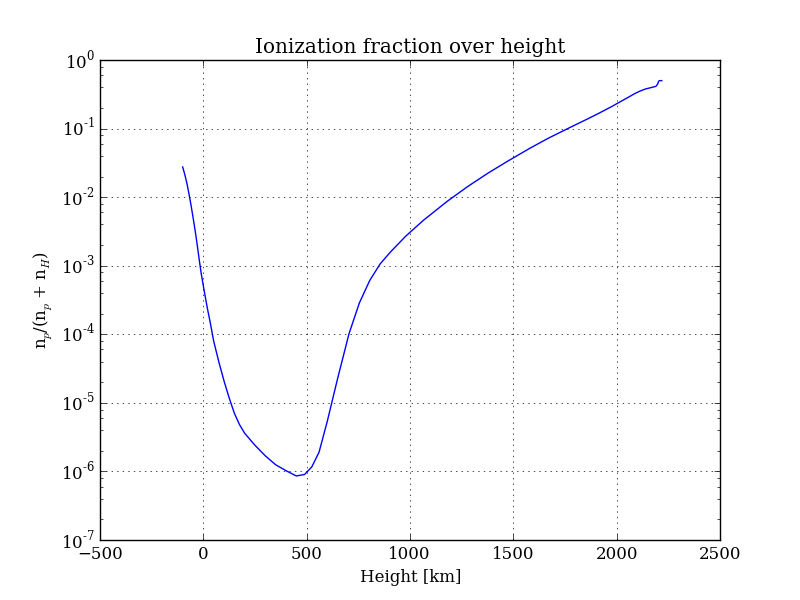
\includegraphics[scale=0.42]{../figs/ion_frac.png}
	\caption{Plot of hydrogen ionization fraction over height.\\
	Ionization, for these conditions in the Sun's hot gas environments, is directly tied to the thermal energies, and thus to temperature - however, not in a linear way: the logarithmic nature of ionization number density is tied to the linear nature of temperature.}
\end{figure}

\subsubsection{Photon densities}
Considering the temperature stratification in figure 1, the gas density and pressure in figure 5 and 6(a), one may observe that the curves all follow the same nature in decreasing, around the deepest parts of the atmosphere. This suggests LTE conditions, and the equation for isotropic radiation given in the assigntment is then applicable, as per requiring a thermal equilibrium to work.

The photon density at this point, the lower height, and its relation to the hydrogen density yield these numbers:
\begin{align*}
N_{\gamma,low} &= 1.661168 \cdot 10^{13} [1/cm^3]\\
\frac{N_{\gamma,low}}{N_{hyd,low}} &= 1.22958 \cdot 10^{-4}
\end{align*}
In other words, the photon density seems negligible compared to the hydrogen density. This suggests itself to be a feature of LTE.

Higher up in the atmosphere, at around 1000 km up, one may see from these graphs that the values drop too much (a factor of around 10$^6$ for density and pressure), and start behaving in different ways, as aforementioned in the density comparison's section, section 1.2.6 - not to mention that the temperature increases wildly, in spite of the pressure and the densities still dramatically decreasing. This sugggests that there are different phenomena that govern the physical nature of these regions, as LTE doesn't seem to apply; at these physical conditions the particles do not interact in the way of LTE.

The photon density at this point, the higher height, and its relation to the hydrogen density yield these numbers:
\begin{align*}
N_{\gamma,high} &= 6.11473396401 \cdot 10^{11} [1/cm^3]\\
\frac{N_{\gamma,high}}{N_{hyd,high}} &= 109.681
\end{align*}
At this point, the hydrogen density is indeed very much lower than that of the photon density, a reversal from the lower height's physical conditions.

The medium there is insensitive to any OTHER wavelength than the Ly$\alpha$ line, because these the Ly$\alpha$ line is a resonant line for the hydrogen atom - as such the hydrogen atoms there will be able to absorb and emit this wavelength naturally, but other wavelengths do not show themselves because the density is too low for any other phenomena than the Ly$\alpha$ emissions to occur, meaning that the hydrogen particles are too far apart from another .


\subsection{Comparison with the Earth's atmosphere}
\subsubsection{Plots of data}

\begin{figure}[H]
\center

	\begin{subfigure}[t]{0.49\textwidth}
	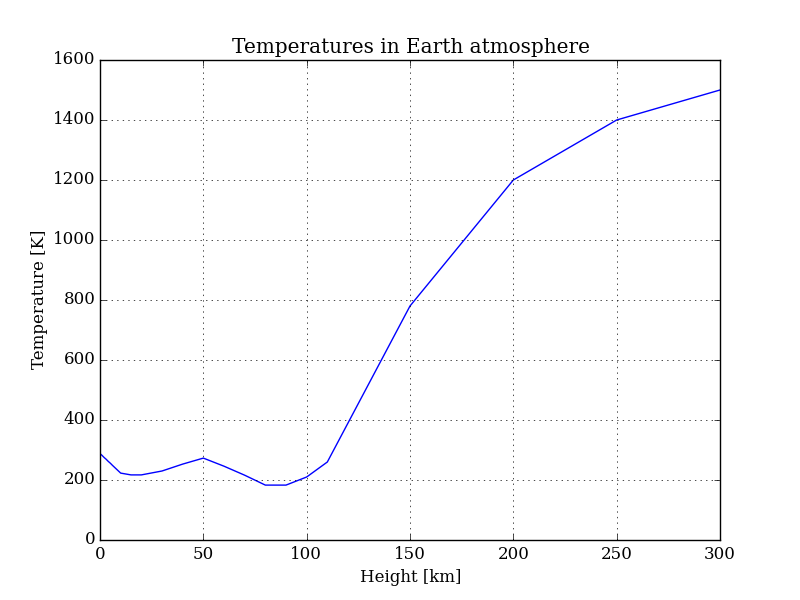
\includegraphics[scale=0.42]{../figs/earth_temp.png}
	\caption{Earth's temperature variation over height.}
	\end{subfigure}
	\hfill	
	\begin{subfigure}[t]{0.49\textwidth}
	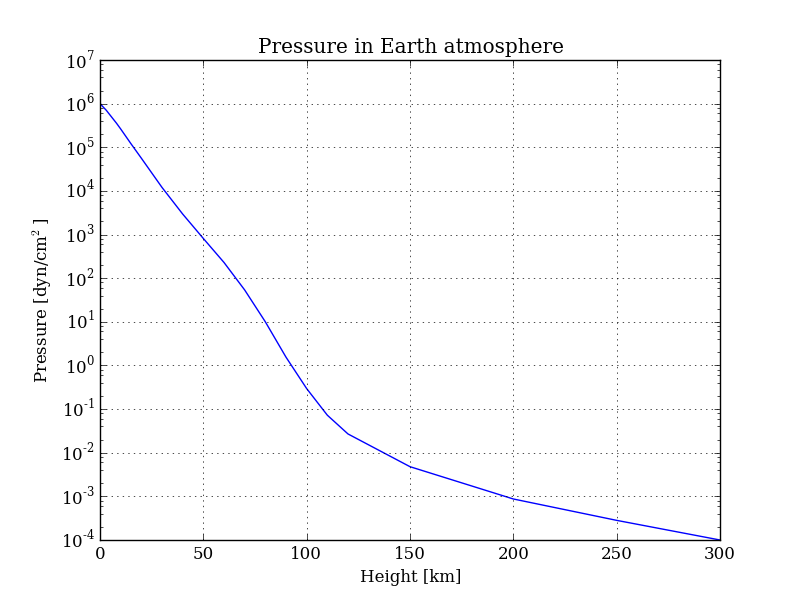
\includegraphics[scale=0.42]{../figs/earth_pressure.png}
	\caption{Earth's pressure variation over height, log scaled.}
	\end{subfigure}\\
	\begin{subfigure}[t]{0.49\textwidth}
	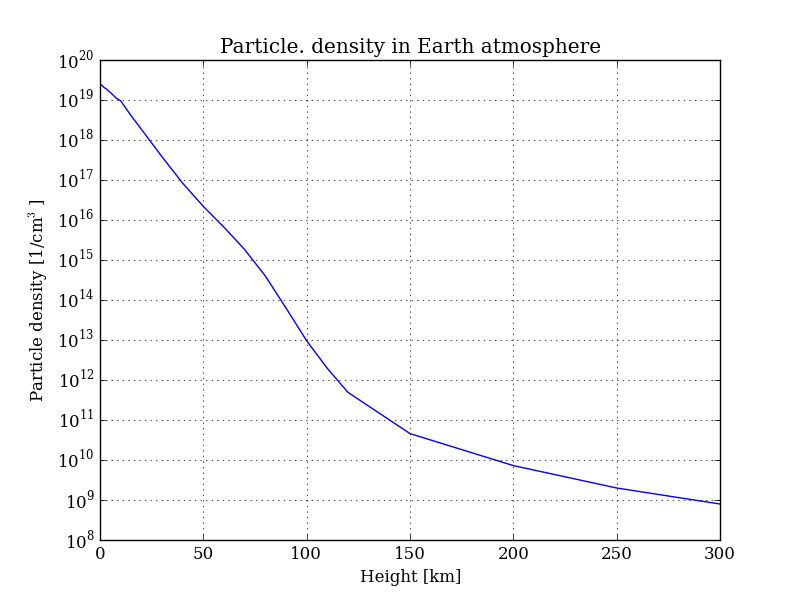
\includegraphics[scale=0.42]{../figs/earth_pardens.png}
	\caption{Earth's particle density variation over height, log scaled.}
	\end{subfigure}
	\hfill
	\begin{subfigure}[t]{0.49\textwidth}
	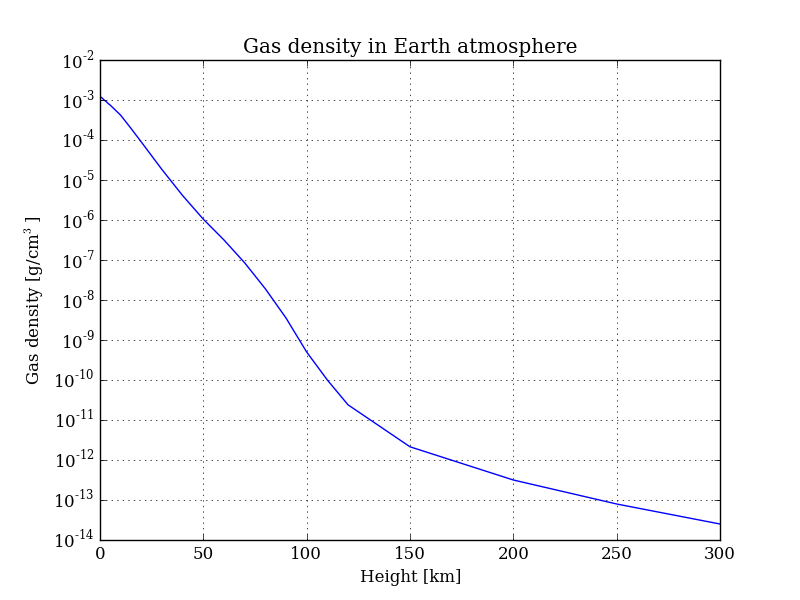
\includegraphics[scale=0.42]{../figs/earth_gasdens.png}
	\caption{Earth's gas density variation over height, log scaled.}
	\end{subfigure}
	
\caption{}
\end{figure}

\subsubsection{Normalized pressure, gas and number densities}
\begin{figure}[H]
\center

	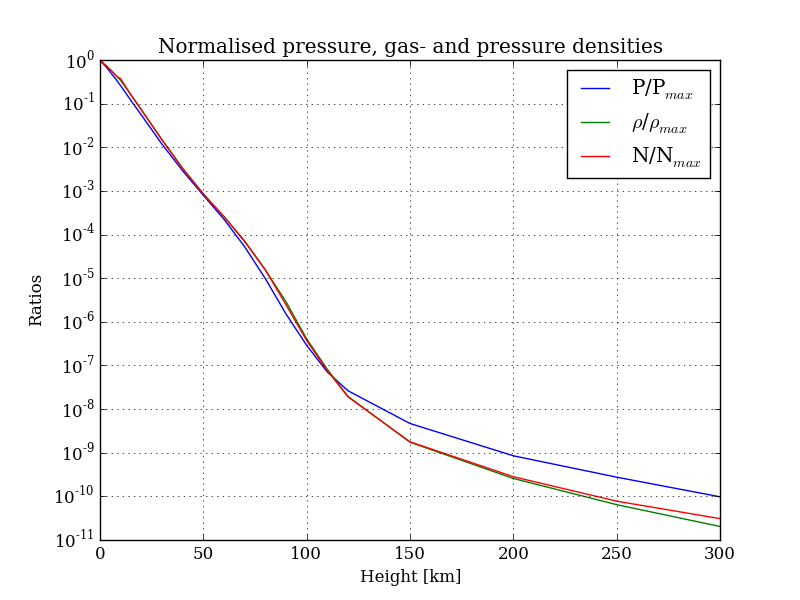
\includegraphics[scale=0.42]{../figs/earth_pres_dens_vs_h.png}
	\caption{Plot of normalized pressure, gas and number densities, over height.\\
	They seem to be decreasing in an intuitive fashion, although the slope of the logarithmic curve seems to change around a height of 120 km, indicating that conditions change in the environment.}
\end{figure}

\subsubsection{Mean molecular weight}
\begin{figure}[H]
\center

	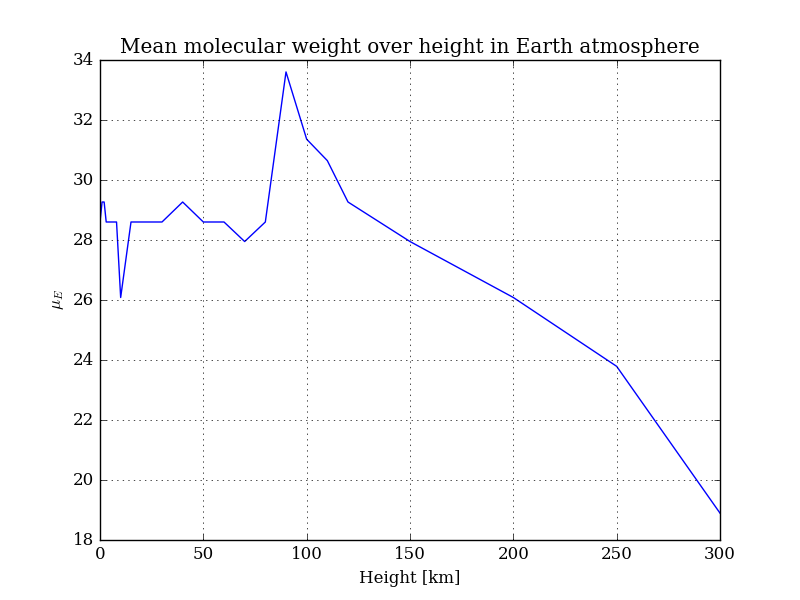
\includegraphics[scale=0.42]{../figs/earth_meanmolweight.png}
	\caption{Plot of mean molecular weight over height.\\
	The mean molecular wieght seems to decrease in higher altitudes above the earth, indicating that there is less significantly less atmosphere to constitue an atmosphere out of. This is fairly intuitive as well, considering how many orders of magnitude the particle density of figure 9 (c) has decreased up until a height of around 120 km.}
\end{figure}

\subsubsection{Earth density scale height}
\begin{figure}[H]
\center

	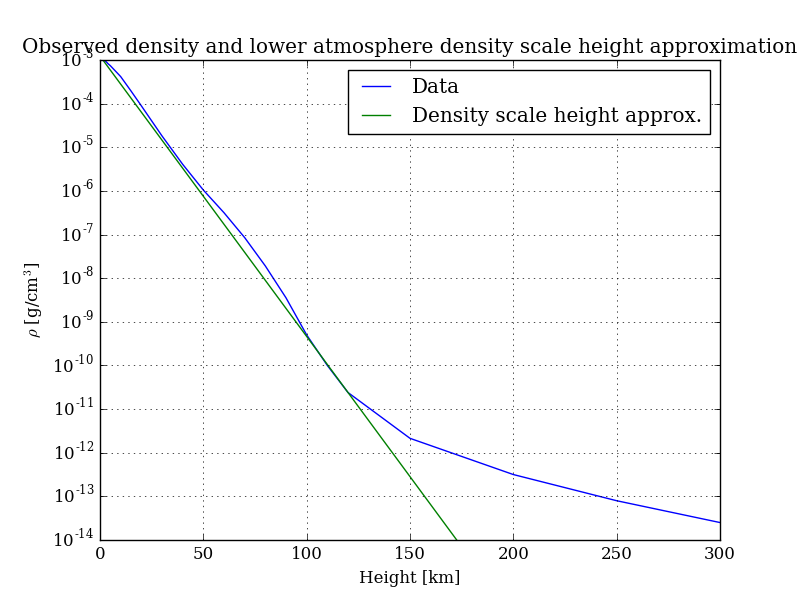
\includegraphics[scale=0.42]{../figs/earth_densityscales.png}
	\caption{Plot of earth atmospheric density and its scale height approximation, over height.\\
	The earth density scale height was calculated in a similar fashion as the solar density scale height. It is applicable over a significantly lesser area than the solar density scale height, at least in proportion to total amount of data.\\
	Given the fact that Mount Everest is at a height less than 10 km up in the atmosphere, and if we assume gases are homogeneously mixed for that area of the earthen atmosphere as they are on the surface, one could easily assume that the human lungs are still capable of taking up enough oxygen from the atmosphere at Mount Everest's peak to biologically function (ignoring the fact that most mountaineers need oxygen supplies along the way up).\\
	If all of this is assumed, one would estimate that the lungs of a mountaineer would have to breathe less than an order of magnitude harder than they normally do on the planet surface.}
\end{figure}

\subsubsection{Earth and Sun surface parameter comparison}
Variable ratios of Earth / Sun on their respective surfaces:
\begin{align*}
\frac{\text{T}_{\text{Earth,surf}}}{\text{T}_{\text{Sun,surf}}} &= 0.0442 \\ 
\frac{\text{P}_{\text{tot,Earth,surf}}}{\text{P}_{\text{tot,Sun,surf}}}   &= 8.4780 \\
\frac{\rho_{\text{tot,Earth,surf}}}{\rho_{\text{tot,Sun,surf}}}    &= 4439.8\\
\frac{n_{\text{tot,Earth,surf}}}{n_{\text{tot,Sun,surf}}} &= 197.48\\
\frac{m_{c,\text{Earth,surf}}}{m_{c,\text{Sun,surf}}}   &= 236.94
\end{align*}

\subsubsection{Solar irradiance at Earth}
Doing the calculations, one yields that the Earth receives a photon density from the Sun
\begin{align*}
N_{\gamma, \text{Sun2Earth}} &= 4.154 \cdot 10^7 [1/cm^3]\ , \intertext{which we may compare to the particle density of our atmosphere:}
\frac{N_{\gamma, \text{Sun2Earth}}}{N_{\text{particle,Earth}}} &= 1.616\cdot 10^{-12}\ , \intertext{or compare with Earth's own low-thermal signature, using the same LTE approximation form as previously in section 1.2.8 for the lower part of the Sun's atmosphere:}
\frac{N_{\gamma, \text{Sun2Earth}}}{N_{\gamma, \text{Earth}}} &= 0.087 
\end{align*}
The last fraction's yielded number would suggest that the Earth is an intensely bright object. While that may well be for the infrared part of the spectrum, it would seem more likely that the Sun does in fact overpower the Earth's own thermal photon production, and that the the lower part of Earth's atmosphere doesn't approximate well to LTE conditions.

%Nphot_atEarth/Npart_fromEarth = 0.087

%Nphot_atEarth/Nphot_atSun     = 6.79408056302e-05



\section{Continuous spectrum from the solar atmosphere} 				%%% section 2

\subsection{Observed solar continua}

\subsubsection{Spectral distribution data}
\begin{figure}[H]
\center

	\begin{subfigure}{0.49\textwidth}
	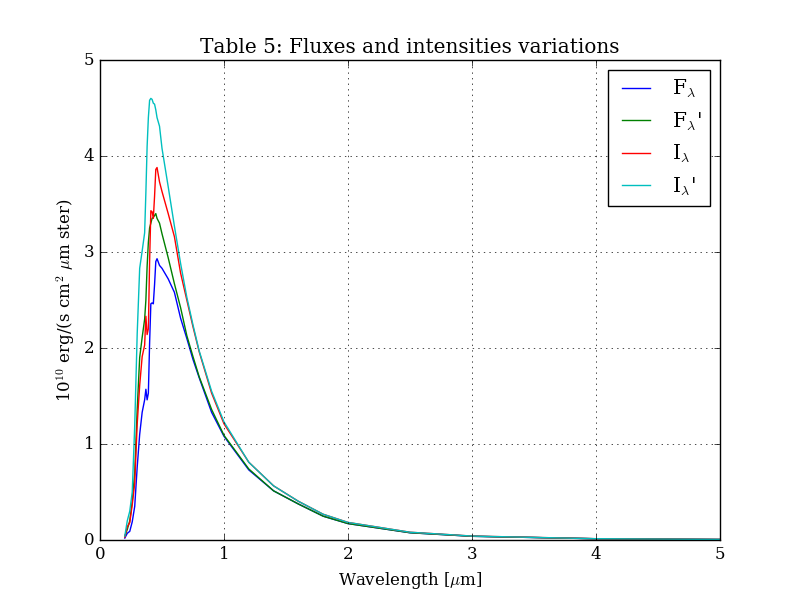
\includegraphics[scale=0.42]{../figs/2obs_sol_cont.png}
	\caption{Plot of the spectral distributions over wavelength.}
	\end{subfigure}
	\hfill
	\begin{subfigure}{0.49\textwidth}
	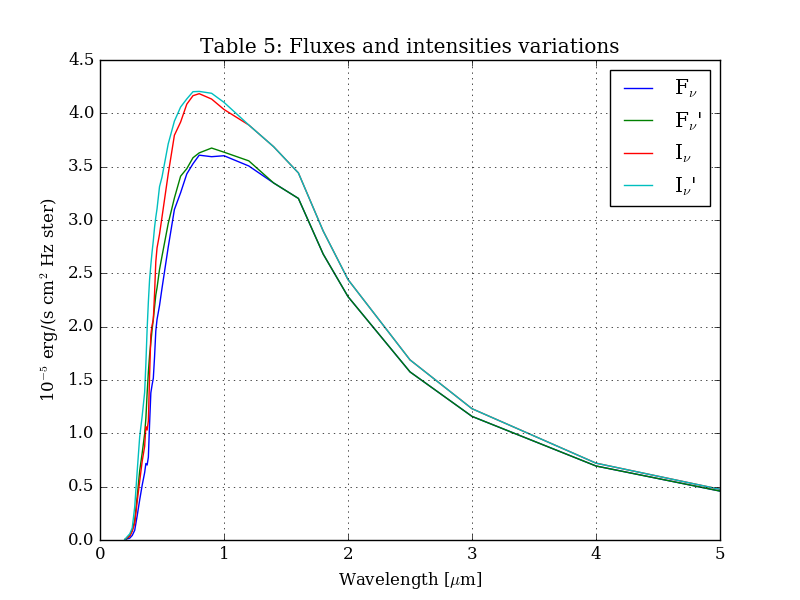
\includegraphics[scale=0.42]{../figs/2obs_sol_cont_freq.png}
	\caption{Plot of the spectral distributions dependant of frequency over wavelength.}
	\end{subfigure}

\caption{Intensity is a measure of flux per solid angle; as such they are intimately connected.}
\end{figure}

\subsubsection{Planck fitting to solar continuum intensity}
\begin{figure}[H]
\center

	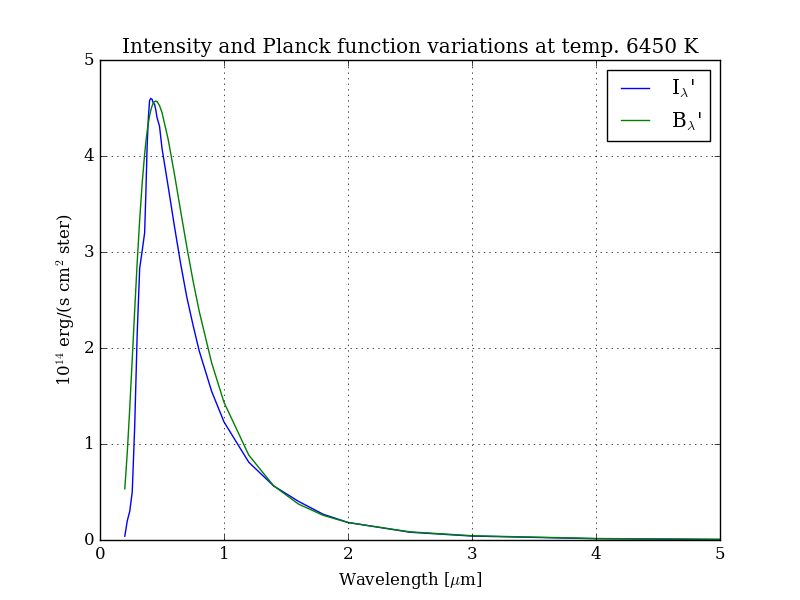
\includegraphics[scale=0.42]{../figs/2obs_planck.png}
	\caption{Plot of intensity distribution over wavelength.\\
	At roughly 6450 degrees K the Planck function fits the observed intensity continuum well.}
\end{figure}

\subsubsection{Brightness temperature distribution over wavelength}
\begin{figure}[H]
\center

	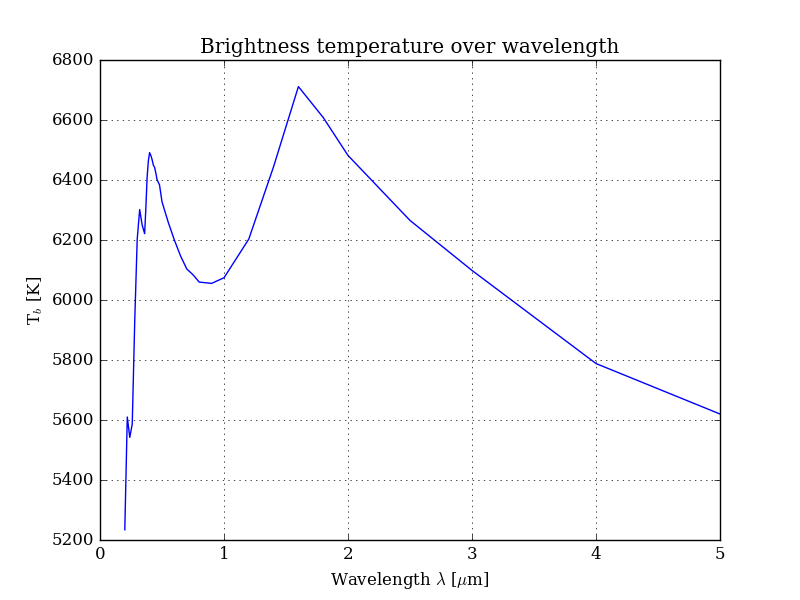
\includegraphics[scale=0.42]{../figs/2obs_Tb.png}
	\caption{Plot of brightness temperature over wavelength.\\
	It almost looks like it's got the shape of a Planck spectral distribution, with the top chopped off and taken a bite out of. This could imply that there is some physical phenomena (i.e. atmospheric absorption and the like) that disturbs the data from which we calculate the brightness temperature.}
\end{figure}

\subsection{Continuous extinction}

\subsubsection{Wavelength variation of hydrogenic extinction for h=0 km}
\begin{figure}[H]
\center

	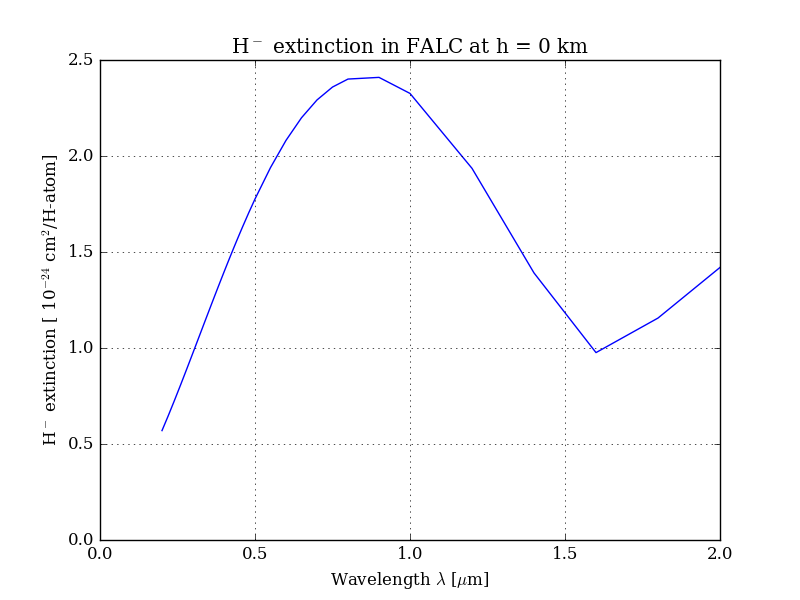
\includegraphics[scale=0.42]{../figs/2cont_ext_gray.png}
	\caption{Plot of ionized hydrogen extinction over wavelength, at $h$=0.\\
	It seems to be identical in shape, although with different magnitudes of units, to Gray's formulation's graphs - in the sense that the above figure's graph follows the summed line of H$^-_{ff}$ and H$^-_{bf}$.\\
	The $bf$ processes behave differently than the hydrogenic ones, becuase the $bf$ transitions require a much higher temperature in order to work.}
\end{figure}

\subsubsection{Extinction line as brightness temperature}
\begin{figure}[H]
\center

	\begin{subfigure}{0.49\textwidth}
	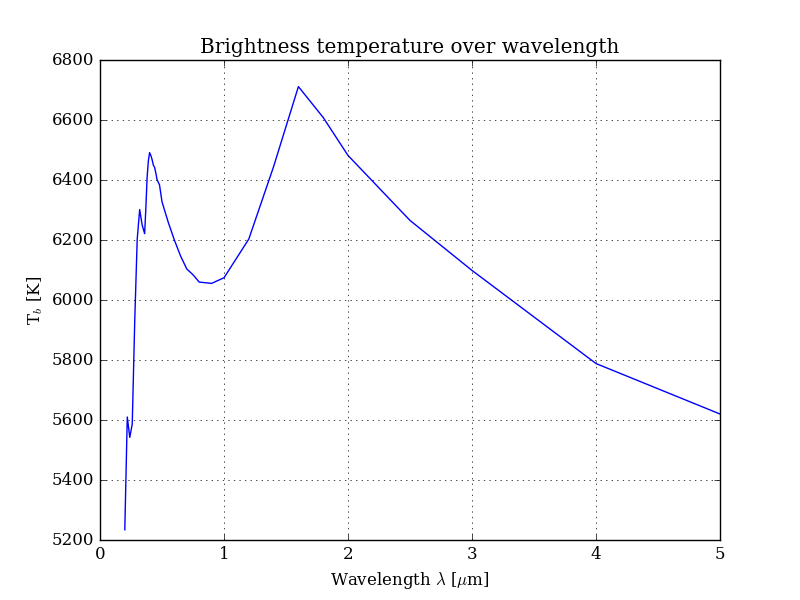
\includegraphics[scale=0.42]{../figs/2obs_Tb.png}
	\caption{Plot of brightness temperature over wavelength.}
	\end{subfigure}
	\hfill
	\begin{subfigure}{0.49\textwidth}
	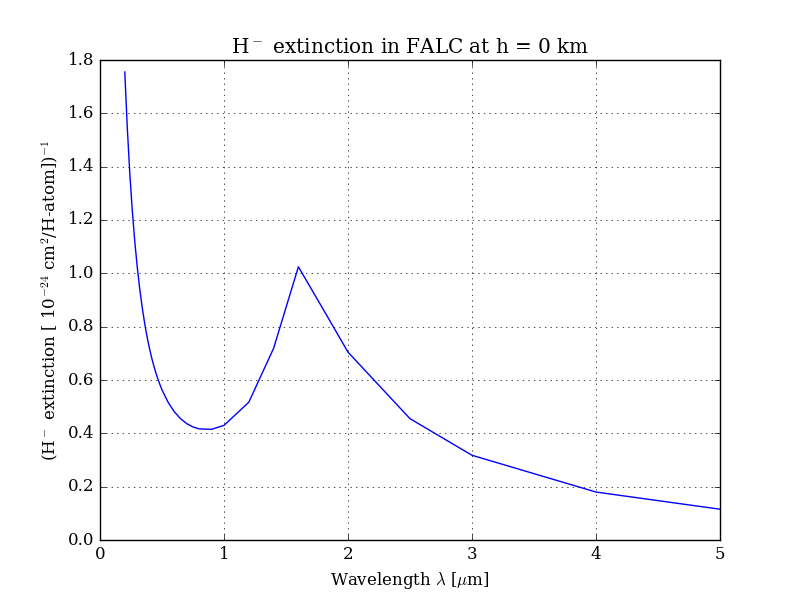
\includegraphics[scale=0.42]{../figs/2cont_ext_Tb.png}
	\caption{Plot of inverted ionized hydrogen extinction over wavelength, at $h$=0 .}
	\end{subfigure}

\caption{Inverting the extinction profile creates a graph that is similar in shape to the brightness temperature over a profile. It is worth noting that the brightness temperature peaks at a wavelength around $\lambda$ = 1.6[nm]. This is the same wavelength at which the H$^-$ inverted extinction has a local peak.}
\end{figure}

\subsubsection{Elements' extinction comparisons}
\begin{figure}[H]
\center

	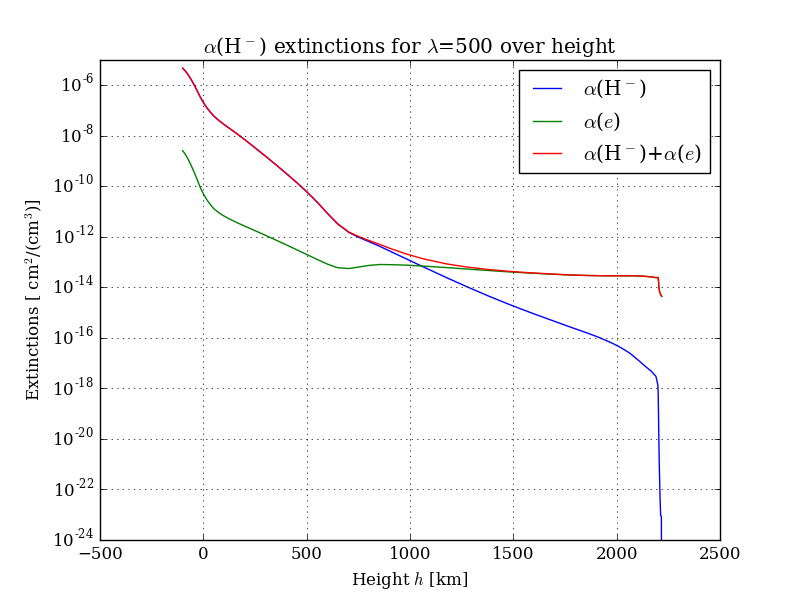
\includegraphics[scale=0.42]{../figs/2cont_ext_over_h_thom.png}
	\caption{Plot of some components extinctions' magnitude for a single wavelength, over height.\\
	It needs to be logarithmic to catch the variations that occur on very small scales.\\
	The Thomson scattering cross section needs to be multiplied with the electron density to yield the necessary extinctions.\\
	At greater heights, it becomes obvious that the Thomson scattering extinction from the electrons' presence in the solar gas, is the dominant part of the total extinction. Conversely, on lower height levels, the extinction is dominated by H$^-$.}
\end{figure}

\subsection{Optical depth}
\begin{figure}[H]
\center
	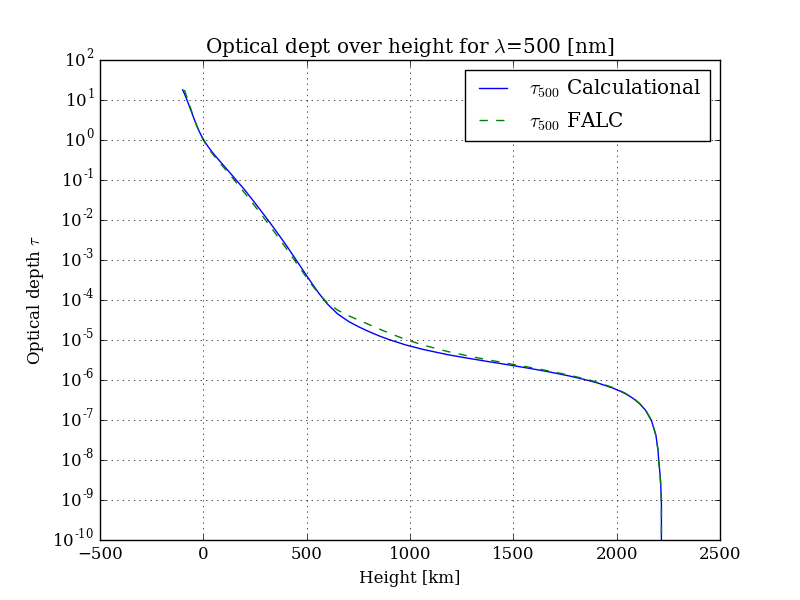
\includegraphics[scale=0.42]{../figs/2opt_depth.png}
	\caption{}
\end{figure}

\subsection{Emergent intensity and height of formation}

\subsubsection{Peak-normalized contribution and peak location}
\begin{figure}[H]
\center
	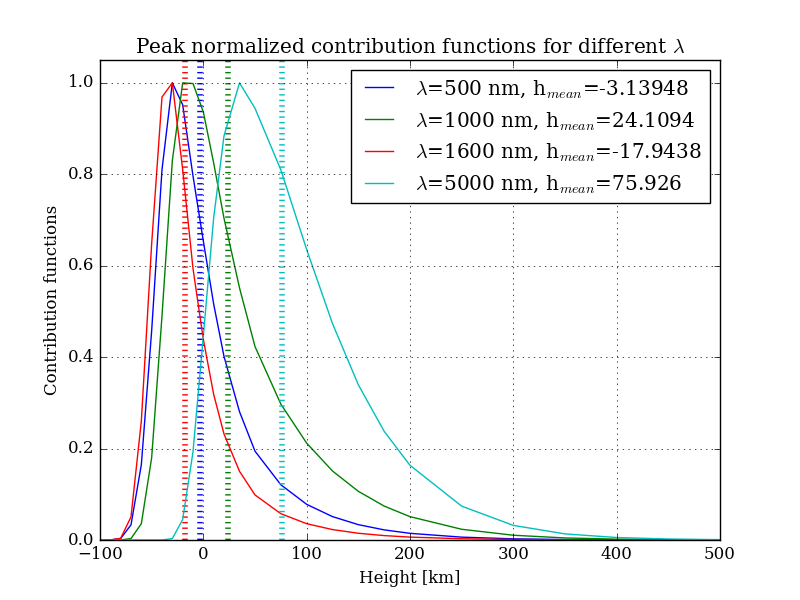
\includegraphics[scale=0.42]{../figs/2emer_peaknormcont_vs_h_wls.png}
	\caption{Plot of the peak-normalized contribution function against height.
	The mean height of formations seems to be off-set from the peak location, at a set amount proportional to features of every wavelengths' curve.}
\end{figure}


\subsection{Disk-center intensity}
\subsubsection{Emergent continuum}
\begin{figure}[H]
\center
	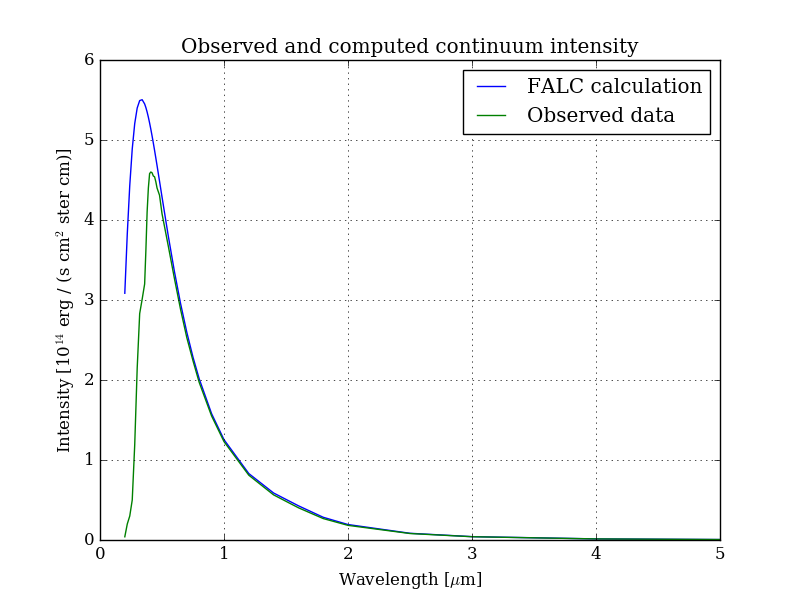
\includegraphics[scale=0.42]{../figs/2disk_center_int.png}
	\caption{Plot of the observed and computed continuum intensity over wavelength.\\
	It seems to fit very well, except for some parts of the spectrum with shorter wavelengths.}
\end{figure}

\subsection{Limb darknening}
\begin{figure}[H]
\center
	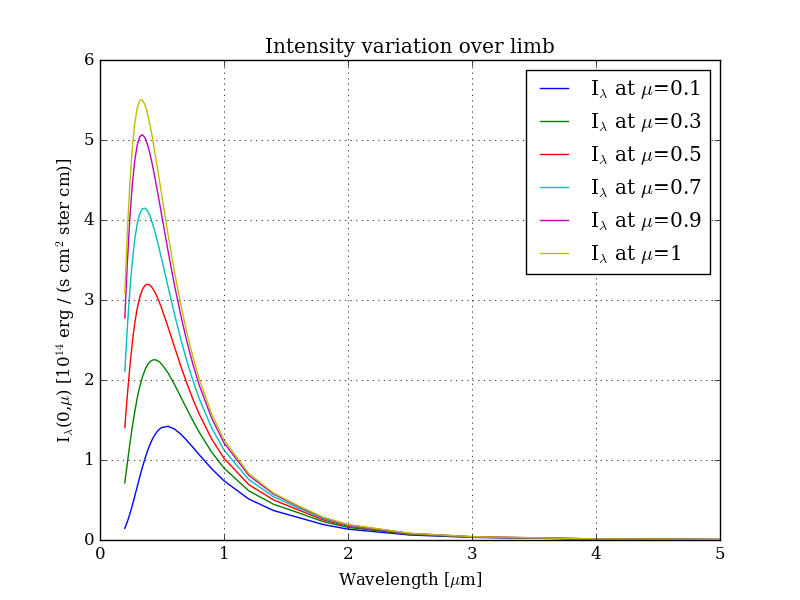
\includegraphics[scale=0.42]{../figs/2disk_limbdark.png}
	\caption{Plot of the observed and computed continuum intensity over wavelength for multiple inclinations of the solar disk.}
\end{figure}


\subsection{Flux integration}

\begin{figure}[H]
\center
	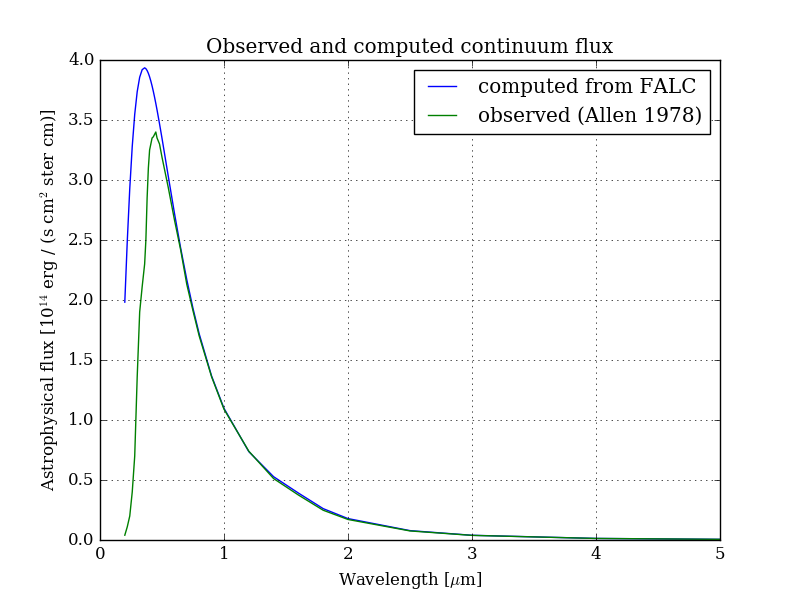
\includegraphics[scale=0.42]{../figs/2flux.png}
	\caption{Plot of the observed and computed continuum fluxes over wavelength. This, too, looks to be a good fit, except for the lower end of the spectrum.}
\end{figure}


\section{Spectral lines from the solar atmosphere} 						%%% section 3

\subsection{Na D wavelengths}
\begin{figure}[H]
\center
	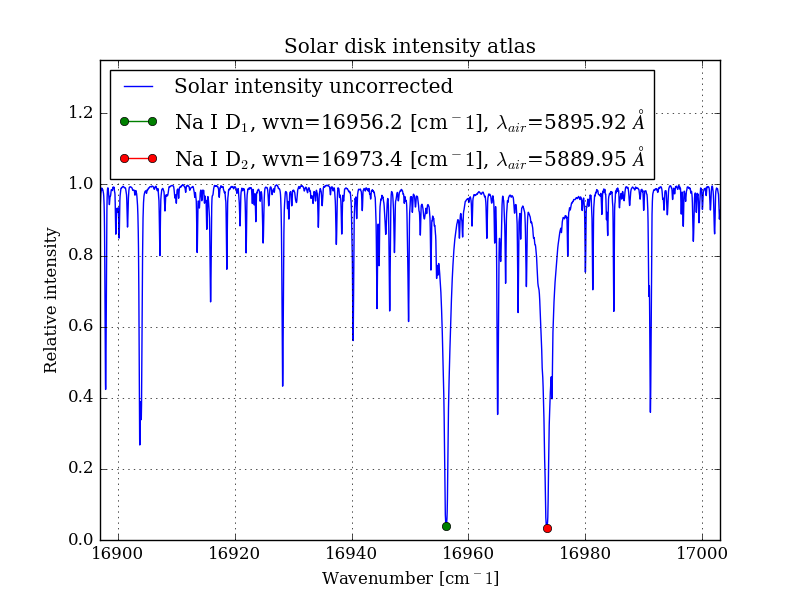
\includegraphics[scale=0.42]{../figs/3vac_wvl_min.png}
	\caption{Plot of relative intensity over wavenumber, from solar intensity.\\
	The NaID lines are noted  by their minima lines at wavelengths $\lambda_{\text{NaID}_1} = 5895.92 \AA$, and $\lambda_{\text{NaID}_2} = 5889.95 \AA$.}
\end{figure}

\subsection{Computed NaID$_1$ line profile}

\begin{figure}[H]
\center
	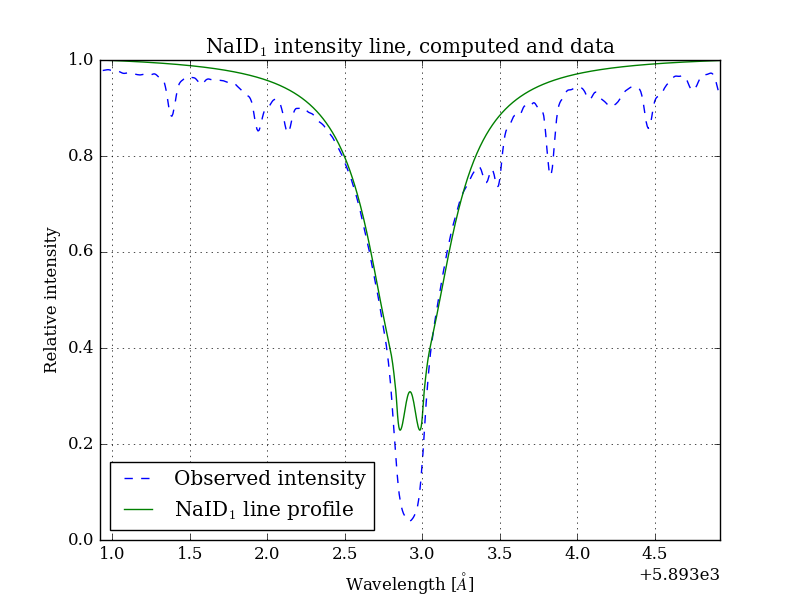
\includegraphics[scale=0.42]{../figs/3NaDspectrum.png}
	\caption{Plot of relative intensity over wavelength, from solar intensity atlas, with computed LTE line profle for NaID$_1$ extinction, using the Unsöld recipe for Van der Waals broading.}
\end{figure}

\subsection{Conclusion/Discussion}
All in all, the whole of this assignment has been about slowly understanding and then adding effects together that together will constitute physical phenomena which we, in the end, may model using programs that include reasonable simplifications for numerical approximations.

In the end, it is impressive how well the numerical model fits, but sadly, it doesn't fit the data completely. This is in large part faulted to some of the assumptions we make, mainly the LTE conditions for the center part of the extinction line - and our numerical model is based on LTE conditions, whereas some physical phenomena that contribute to actual extinction are not.

This is why there is a line center reversal in the computed model's extinction profile, where there should be none. Other than this, the wings seem to fit quite well for the actual Sodium extinction; there are minor discrepencies outside the FWHM-area which are probably results of completely different extinction phenomena than the sodium extinction.

When it comes down to the enhancement factor $E$, I found that the value of $E$ = 2 yielded the best-fitting results.

To be completely honest, the hardest part of this assignment is keeping track of the units of data going into functions; and different functions having different preferences. A solution to this could be to implement the infamous \verb|Astropy| library to let it keep track of units for us - but I chose not to, and did well not to implement \verb|Astropy|. The numerical calculator for flux at the end of section 2 took me 1.1 seconds to read, run and plot. Compared to an \verb|Astropy|-oriented script designed by a student peer of mine, where his program required over a full hour to run with that library, I'm glad I've chosen to understand how these programs interconnect, rather than letting some library fix this for me.

That said, I really wish everything we measured and calculated was measured to SI units, so that I would be able to concentrate on learning the physics behind the models' phenomena, rather than spending hours on end troubleshooting programs that may or may not to what they should, or they may or may not be simply misinterpreting units that we forget to keep track over, given the fact of how intricately interconnected these units indeed are.

\section*{Appendix - Github} \label{section:github}
\url{https://github.com/magnucb/Ast4310-SSB}


\end{document}